\section{Synapsed}

\begin{frame}{Introduction}
	Previous results show that:
	\begin{itemize}
		\item There is high lock contention
		\item The amount of RAM is important
	\end{itemize}
	\dspc
	If cached remains at the host, it will:
	\begin{itemize}
		\item Compete for CPU time
		\item Use a fraction of the host's RAM
	\end{itemize}
	\dspc
	Idea: what if cached ran on storage nodes?
\end{frame}

\begin{frame}
	If cached was on storage nodes, the pros would be:
	\begin{itemize}
		\item Access to more RAM
		\item Major step towards a distributed cache
	\end{itemize}
	\dspc
	On the other hand, the cons would be:
	\begin{itemize}
		\item Network bottleneck
		\item Bigger complexity
	\end{itemize}
	\dspc
	Archipelago is network-unaware. Must create a proof-of-concept network peer 
	to help us in this task.
\end{frame}

\begin{frame}{Synapsed design}
	Synapsed is designed to do the following:
	\begin{itemize}
		\item Connect two Archipelago peers over network
		\item Forward read/write XSEG requests
		\item Use the TCP protocol
		\item Integrate with the Archipelago signaling mechanism
		\item Use zero-copy methods
	\end{itemize}
	\dspc
	Replication should be trivial to implement, but it is currently missing.
\end{frame}

\begin{frame}{Benchmark preamble}
	The most important part is that synapsed works. We are \textbf{now} able to
	run cached or part of Archipelago in the storage nodes.
	\dspc
	However, let's check its performance.
	\spc
	We will attempt to run most of the previous scenarios using synapsed this 
	time.
	\dspc
	Note, synapsed is proof-of-concept and not performance-tuned. Also, the 
	tested configuration uses a 1Gbit connection.
\end{frame}

\begin{frame}{Synapsed results}
	\begin{columns}[t]
		\begin{column}{.5\textwidth}
			Write bandwidth
			\makebox[\textwidth]{
				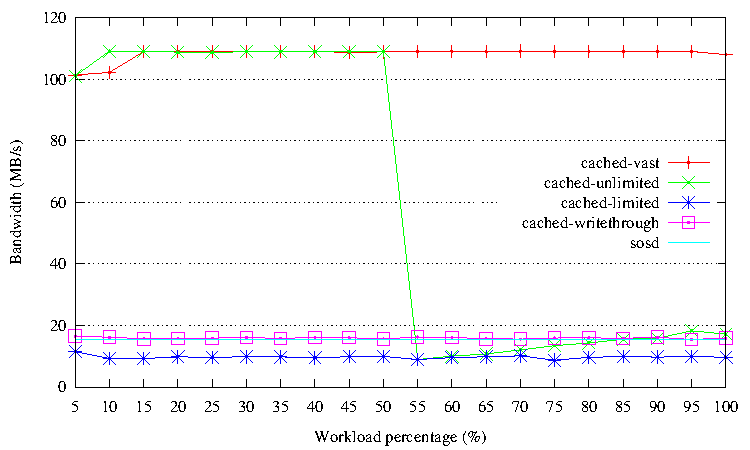
\includegraphics[width=\columnwidth]{images/bw-write-synapsed.pdf}
			}
			Constants:
			\begin{itemize}
				\item cached has 4 threads
				\item workload twice the cache size
				\item block size is 4KB
				\item Parallel requests are 16
			\end{itemize}
		\end{column}
		\begin{column}{.5\textwidth}
			Write latency
			\makebox[\textwidth]{
				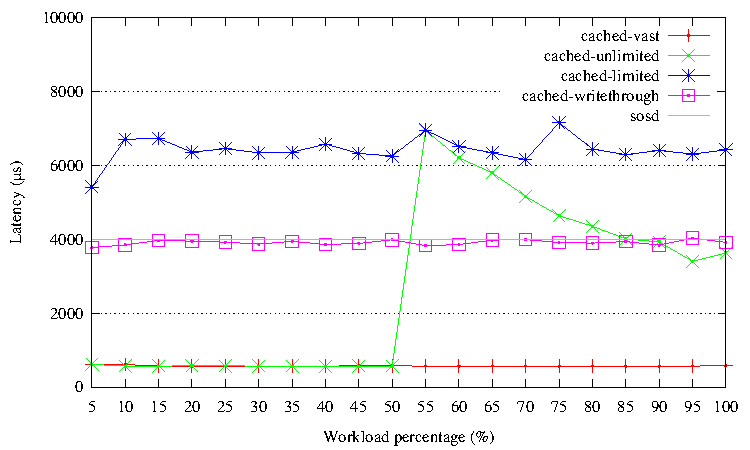
\includegraphics[width=\columnwidth]{images/lat-write-synapsed.pdf}
			}
			Variables:
			\begin{itemize}
				\item cache write policy
				\item maximum cached objects
			\end{itemize}
		\end{column}
	\end{columns}
\end{frame}

